\chapter{Validation de la commande en temps continue sur le modèle non linéaire}
\label{ValidationCommande}
%% Chemin d'accès au répertoire : Conception-de-commande\Implémentation Commande Moteur\AGarder\Commandes_matlab
Maintenant que les étapes de démonstration et de simulation de la commande sur des modèles linéaires sont terminés, nous allons pouvoir créer notre premier prototype, que nous nommerons prototype 0. Il correspondra à notre solution 0. Nous allons d'abord effectuer ce que nous appelons un \emph{Model in the loop} où nous allons chercher à améliorer ce premier prototype en utilisant uniquement des simulations. Par la suite, nous améliorerons le prototype en utilisation une technique d'émulation dite \emph{Software in the loop}.
\section{Protocoles MIL/SIL}\label{sec:prtocoleMIL_SIL}
Dans cette partie, nous allons expliquer les démarches que nous utiliserons pour valider nos prototypes. 
	\subsection{Model in the loop (MIL)}
	Pour faire une validation MIL, nous allons utiliser le modèle non linéaire pour simuler la correction. Toute cette opération sera effectué sous $MATLAB$ à l'aide d'un bloc \emph{SIMULINK} qui simule le modèle non linéaire. Pour valider le prototype de commande du correcteur, celui-ci devra respecter la ou les condition que nous lui imposerons. S'il ce n'est pas le cas, une amélioration de ce prototype sera nécessaire et elle nous permettra de créer un prototype N (pour N itérations de cette boucle). 
%	Nous devons d'abord fixer une marge d'erreur par rapport au cahier des charges défini en \ref{chap:commande} : 
%	\begin{align}\label{eqn_margeErreur}
%		M_\epsilon < 1\%
%	\end{align}
%	Tant que notre prototype ne sera pas en dessous de cette marge, nous devrons le modifier et refaire le test.
	\subsection{Software in the loop (SIL)}
	Après la validation en MIL, nous passerons à une validation \emph{Software in the loop}. Le prototype obtenu au bout de la boucle MIL sera ici testé sur sa partie logicielle. Nous testerons ici si le temps concret de commande est vérifié, en branchant directement le calcul de la commande sur un autre ordinateur ou bien en utilisant un moteur réel. Pour cela, nous n'hésiterons pas à effectuer un prototypage rapide, une fonction de \emph{MATLAB}, qui permet de recevoir et d'émettre des signaux analogiques depuis un ordinateur via un une carte E/S. 
	
	De même que pour le MIL, si le prototype $N$ ne valide pas le cahier des charges, nous devons recommencer le test en créant un nouveau prototype $N+1$ jusqu'à que la commande soit satisfaisante. 
%\section{Test des prototypes des commande à temps continue}
	%	Test des commandes TC sur MNL et Moteur
	% 	Utilisation protocoles MIL  (ne le ré-explique pas)  
	%			The PLAN
	\begin{center}
	A présent, nous pouvons commencer à tester les prototypes de commandes du moteur sur des modèles plus complexe : nous disposons pour cela d'un modèle non linéaire ainsi que d'un banc moteur. Nous suivront les consignes que nous venons de présenter en \ref{sec:prtocoleMIL_SIL}, en commençant par présenter le moyen utilisé pour adapter la simulation. 
	Comme il est évoqué dans le titre de cette section, nous sommes ici en temps continu. Les hypothèses pour la discrétisation ne sont pas traités dans cette partie, nous avons choisi de construire le prototype de commande à temps discret quand nous aurons d'abord validé complètement la commande en temps continu, et que nous auront présenté toutes les contraintes que la discrétisation devra surmonter. 
	\end{center}
	%% TODO - ref vers parti discrétisation.
	\section{Simulation sur Modèle Non linéaire}
		
		Nous disposons de la démarche que nous allons utiliser pour valider notre simulation. Pour cette partie, nous utiliserons un bloc \emph{SIMULINK} qui nous permettra de simuler un modèle très proche du banc moteur. Ce modèle n'a pas reçu les simplifications que posent les hypothèses faites en \ref{sub:linearisation} et en \ref{sub:invariance}. Un bloc \emph{SIMULINK} est disponible à cet effet, sous forme de \emph{S-Function}. Il utilise la modélisation et les paramètres utilisés en \ref{sub:equationPhysique} pour créer un système Entrées/Sorties beaucoup plus proche que le modèle linéaire d'ordre 4. 
		% Image et mesure
		%\subsubsection{Adaptation modèle}
		\subsection{Adaptation modèle}
		% Encapsulation de la commande ?
		Pour permettre l'utilisation de ce modèle, nous devons d'abord lancer une compilation de la \emph{S-function}. Cette opération est nécessaire car la \emph{S-function} est un code en langage C qui s'adapte à la simulation \emph{SIMULINK}, et êrmet ainsi d'obtenir des performances en temps de calcul plus élevé qu'en bloc de simulation classique.
		Nous avons choisi d'en-capsuler tout le bloc de commande (Gain du retour d'état et reconstruction d'état) dans un bloc \emph{sub-system} que nous détaillons en annexe \ref{annex:modl_NL_SIMULINK}. Ce sous bloc prend en entrée 2 signaux : la consigne de référence $y_ref$ et la sortie mesuré du système $y_m = V_s$ (Position du moteur, cf chapitre \ref{chap:modelisation}), et calcule la commande qu'il émet sur le connecteur nommé $u$.
		\begin{figure}[ht]
		\centering
		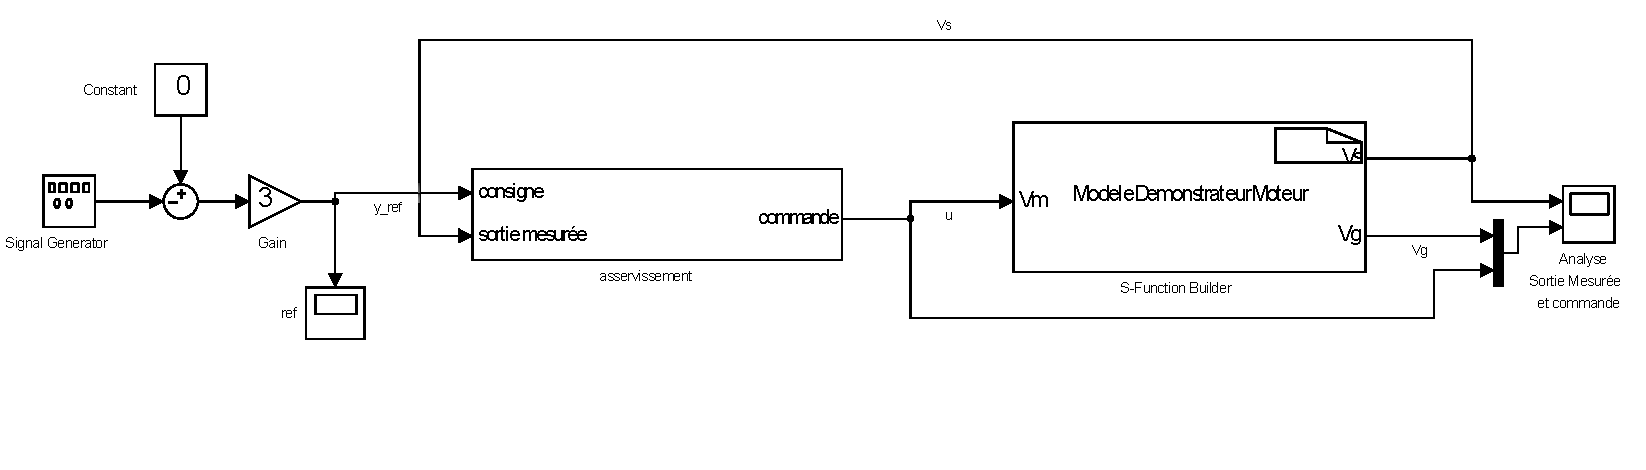
\includegraphics[width = \textwidth]{./IV/images/NL_RE_BlocEntier.pdf}
		\caption{Schéma \emph{SIMULINK} complet de l'asservissement du modèle du moteur Non linéaire}\label{fig:SIMULINK_NL_schema}
		\end{figure}
		
		Nous avons placé des points de mesure au sur le signal de référence ainsi qu'en sortie du système. Nous obtenons ainsi une réponse temporelle que nous allons étudier dans la sous section suivante.
		%\subsubsection{Simulation et étude de performances}
		\subsection{Simulation et étude de performances}	
		%\paragraph{Nouveau paramètres non linéaire}
		\subsubsection{Nouveau paramètres non linéaires}
		Utilisons maintenant la simulation précédente pour étudier les performances de notre commande. Nous avons dans un premier temps observé la reconstruction d'état du système et nous avons pu noter un problème. Un premier problème apparait, nous avons un nouveau paramètre que nous n'avons pas modélisé dans les parties \ref{chap:modelisation} et \ref{chap:analyse}. 
		
			
		Cette nouvelle dynamique correspond à la mesure de la position du moteur : elle se retrouve être borné entre $[-5V; +5V]$ qui correspond aux limites des tensions générés par le banc moteur. Si elle dépasse l'un des seuils, elle est immédiatement retranscrite sur le seuil opposé. Nous pouvons représenter ce phénomène avec le système d'équation suivant :
		\begin{align*}
		V_s(t) = \left\lbrace \begin{aligned}
		&K_rK_s\theta_s \text{ si } \theta_s \in \left[\frac{-5}{K_rK_s}; \frac{+5}{K_rK_s}\right]\\
		&-5 \text{ si } \theta_s < \frac{-5}{K_rK_s}\\
		&+5 \text{ si } \theta_s < \frac{+5}{K_rK_s}
		\end{aligned}
		\right.		
		\end{align*}
		La non linéarité de cette dynamique a été enlevé lors de la modélisation du système en modèle linéaire. Cela pose un problème pour la reconstruction de la vitesse par rapport à la position : nous avions remarqué en \ref{sub:observateurSurModelO4} et en \ref{eqn:erreurRecompoOrdreSup} que lorsque l'observateur(pour l'ordre 2) était implémenté sur des modèle d'ordre supérieur, la dynamique de l'erreur de reconstruction n'était pas uniquement dépendante de lui même, les états non présents dans le modèle d'ordre 2, i.e. les 2 courants $i_1$ et $i_2$, ajoutent un décalage dans la reconstruction des états $\omega$ et $\theta$.
		% Convergence rrapide 
		
%\paragraph{Prototype 0}			
\subsubsection{Prototype 0}
Avec tous ces éléments, nous sommes capables d'expliquer pourquoi les résultats obtenus pour les valeurs propres décidées dans les parties précédente donnent une reconstruction trop erroné de l'état du système. La reconstruction de la vitesse par rapport à la position qui est renvoyé vers l'opposé à chaque dépassement de $[-5;5]$ avec les valeurs propres de l'observateur placé en $3\times v_{p_{des}}$ (cf \ref{sub:constructionObeservateur}) donnent une restitution décalée, qui converge très mal et qui donc ne peut pas être utilisé pour calculer une commande. La non linéarité apparait, pour une consigne de vitesse de $3V$, à peu près 4 fois par seconde. L'observation de la réponse de ce prototype est disponible sur la figure \ref{fig:repNL_proto0}. Dans cette réponse temorelle, le gain K est donnée par le vecteur suivant :
\begin{equation}\label{eqn:gainRetourEtat}
K = \begin{pmatrix}
0& 0.089
\end{pmatrix}
\end{equation}
Pour rappel, nous annulons le retour de l'état de position pour asservir le moteur en vitesse uniquement. (cf \ref{sub:constructionAsservissement}).
\begin{figure}[!ht]
\centering
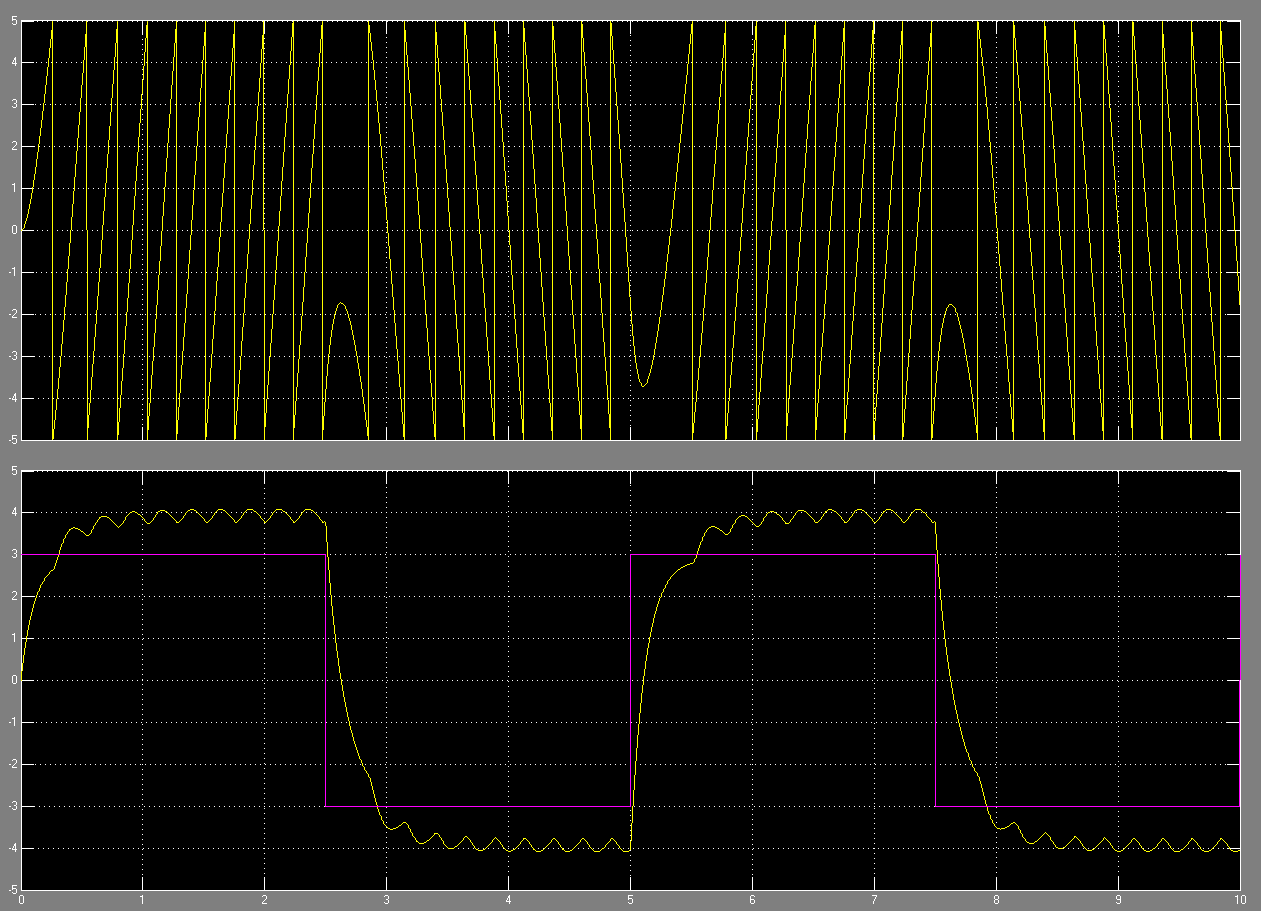
\includegraphics[width = .8\textwidth]{./IV/images/NL_simulation_observateurtropRapide.PNG}
\caption{Simulation réponse temporelle du modèle linéaire commandé par le prototype 0\label{fig:repNL_proto0}}
Simulation des signaux $V_s$ (Bloc du haut), de $y_{ref}$(Bloc du bas/courbe violet) et de $V_m$(Bloc du bas/courbe jaune)
\end{figure}
Nous observons sur cette figure que le changement de seuil de la tension $V_s$ fausse totalement la reconstruction de la vitesse. Pour minimiser l'erreur sur ce modèle, nous devons faire coller les valeurs propres de l'observateur avec celles du système en boucle fermé. Cela devrait réduire les effets non linéaires de la sortie $V_s$. Nous choisissons de commencer l'étude d'un nouveau prototype.

%\paragraph{Prototype 1}
\subsubsection{Prototype 1}
Nous avons changé les valeurs propres de l'observateur pour les faire correspondre avec les valeurs propres désirés. 		
		% Changement des valeurs propres.
			
		% Nouvelle simulation.
Une nouvelle simulation faite sur ce nouveau prototype nous donne les résultats montré dans la figure \ref{fig:fig:repNL_proto1}. Nous pouvons voir une erreur sur le régime permanent qui subsiste toujours. Ce léger décalage devrait pouvoir être corrigé sur un modèle linéaire avec un ajout d'un gain pur compenser ce manque. Or, nous sommes sur un modèle non linéaire et cette méthode ne peut pas fonctionner.


Un zoom sur l'erreur du régime permanent, disponoble en annexe \ref{annex:modl_NL_SIMULINK} - figures \ref{fig:SIMULINK_NL_erreur_reponse} et \ref{fig:SIMULINK_NL_erreur_reponse_zoom}, nous indque que pour une consigne $y_{ref} = 3$, nous obtenons $V_m(t_f)\approx 2.85$. Nous avons donc une erreur en régime statique \begin{align*}
\epsilon_y = y_{ref}-V_m(t_f) = 0.15 \text{, qui correspond pour la consgne demandée à : } \epsilon = \frac{\epsilon_y}{y_{ref}}5\%
\end{align*}
Avant de terminer l'analyse de ce prototype, nous nous intéressons au signal de commande envoyé sur l'émulation du moteur. Celle ci se trouve dans la figure \ref{fig:comNL_proto1}. 

\begin{figure}[!ht]
\begin{minipage}{.5\textwidth}
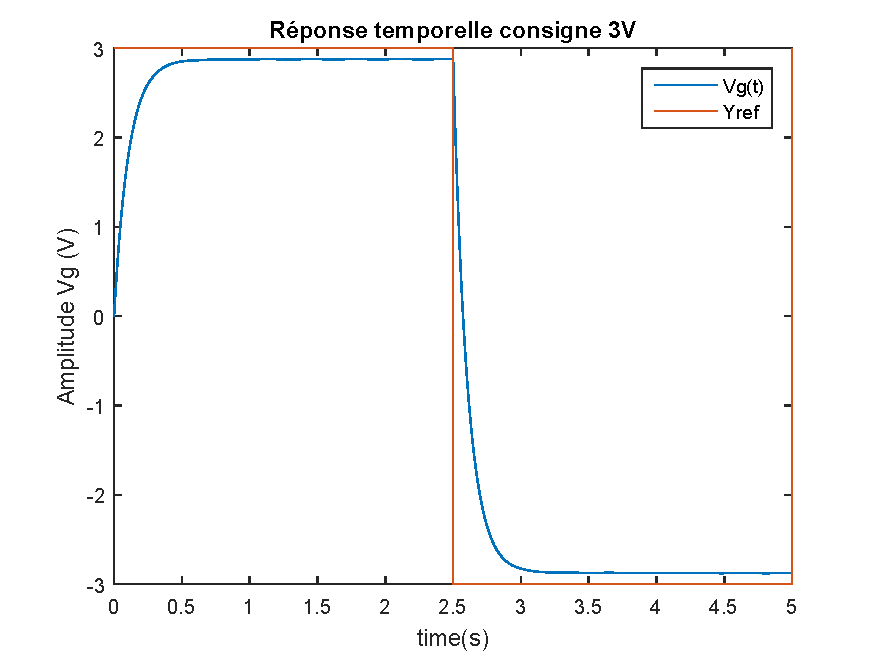
\includegraphics[width= .8\textwidth]{./IV/images/repNL_proto1.pdf}
\caption{Simulation réponse temporelle du modèle linéaire commandé par le prototype 1\label{fig:repNL_proto1} }
\end{minipage}
\begin{minipage}{.5\textwidth}
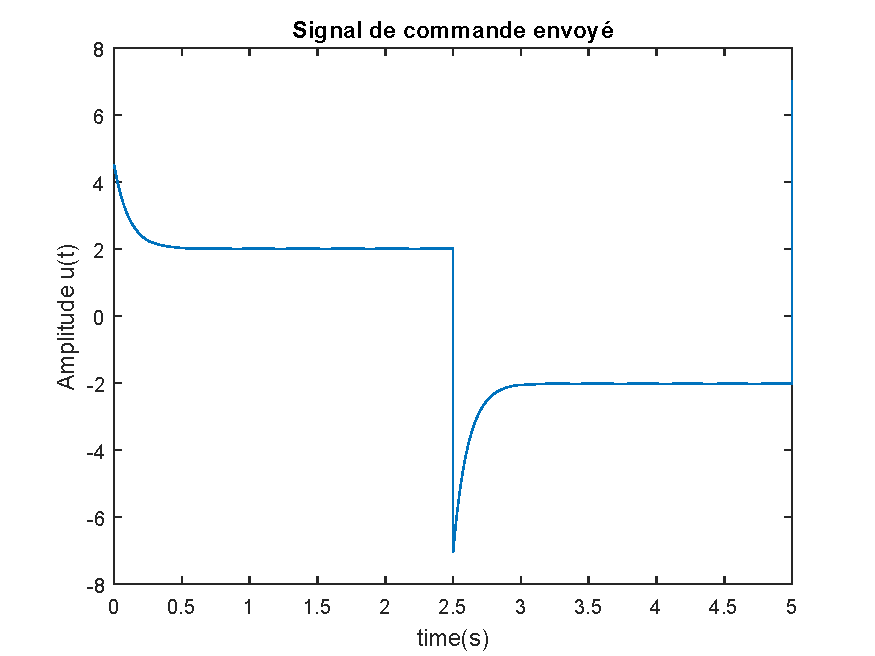
\includegraphics[width = .8\textwidth]{./IV/images/comNLproto1.pdf}
\caption{Simulation signal de commande modèle non linéaire avec le prototype 1\label{fig:comNL_proto1}}
\end{minipage}
\end{figure}  
La commande a une amplitude supérieur à celle de la référence, nous sommes donc dans un asservissement tel que la référence ne peux pas demander la vitesse maximale du moteur. En effet, si la référence demande une vitesse du moteur qui amène un signal de commande dépassant la tension maximale, la vitesse ne sera plus asservi par la commande, et nous serons dans un cas non déterminé où nous n'avons aucune possibilité de savoir si le cahier des charges sera respecté.
Nous décidons de passer à l'implémentation d'un nouveau prototype. Ce prochain prototype devra corriger l'erreur de position ou du moins la minimiser et il devra vérifier que la commande ne dépasse pas le seuil maximal de la référence, pour un temps de réponse toujours dans les close du cahier des charges.

\begin{center}
\textit{Nous proposons de modéliser un nouveau prototype de commande en réutilisant le retour d'état et en ajoutant une action intégrale.}
\end{center}
%\subsection{Retour d'état avec action intégrale}
\section{Retour d'état avec action intégrale}
		Ce nouveau prototype de commande va calculer un nouveau retour d'état, en utilisant cette fois ci la différence entre la référence et la sortie mesurée du système. Pour sa construction, nous nous référons au cours du Master ISTR EEA sur la construction d'un retour d'état. 

		
Dans cet asservissement, un nouvel état du système noté $x_i$ apparait dans la chaine directe. Il est décrit par la dynamique suivante :
		\begin{equation}\label{eqn:dynamique_Xi}
		\dot{x}_i = y_{mes} - y_{ref}
		\end{equation}
		Ainsi, cet état dépend directement de la mesure et de la référence. Les équations du reste de l'espace d'état sont inchangés, et ainsi nous pouvons obtenir une nouvelle représentation d'état donnée avec comme vecteur d'état $X(t) = \begin{pmatrix}
		x & x_i
		\end{pmatrix} = \begin{pmatrix}
		\theta & \omega & x_i
		\end{pmatrix}$
\begin{equation}\label{eqn:EERetourIntegral}
\dot{X} = \begin{pmatrix}
A&0 \\ C& 0
\end{pmatrix}X(t) + \begin{pmatrix}
B \\ 0
\end{pmatrix}u(t) + \begin{pmatrix}
0 \\ -1
\end{pmatrix}y_{ref}
\end{equation}		
		
Nous posons ensuite la nouvelle loi de commande :\begin{equation}
		\label{eqn:loideCommande_retourIntegral}
		u(t) = -K_ix_i(t) - K_px(t)
\end{equation}
		Le gain $K_i$ est le gain intégral associé à $x_i$ et le gain $K_p$ correspond au gain du retour d'état précédemment établi. Ces gains seront calculés comme un placement de pôle, avec la fonction \emph{place}, une fois que les valeurs propres sont choisies. Pour celles ci, nous voulons appliquer la même dynamique que celle étudié en \ref{sub:Calcul du retour etat} en plus de la nouvelle (pour $x_i$). Les valeurs obtenu pour les gains sont les suivantes :
		\begin{align}
		K_p &= \begin{pmatrix}
		0&0.5825  
		\end{pmatrix}\\
		K_i &=  28.5507
 		\end{align}
 		Nous annulons encore le retour de la vitesse dans la chaine directe. Nous allons maintenant effectuer des simulations de ce nouveau retour sur le modèle linéaire. Une fois les simulations validés, nous pourrons passer à la validation de ce nouveau prototype sur un modèle non linéaire.
		%\subsubsection{Simulation de l'action intégrale sur modèle linéaire et non linéaire}
		\subsection{Simulation de l'action intégrale sur modèle linéaire et prototype sur modèle non linéaire}
		Les simulations que nous avons effectué de ce retour d'état ont été faites uniquement sur le modèle linéaire d'ordre 4 qui est, de par son ordre, le plus complexe des modèle linéaire à notre disposition. Nous avons effectué les simulations avec l'environnement \emph{SIMULINK}, le schéma du retour est disponible en annexe \ref{Annex:SIMULINK_RE}, figure \ref{fig:sousSystemeRI}. Dans ces schémas, nous n'avons pas mesuré la vitesse du moteur, nous l'avons reconstruit. Le signal de $y_{mes}$ ne peut pas être la vitesse car inaccessible au mesure. Nous sommes donc obligés de reconstruire ce signal, via l'observateur en utilisant $\hat{x}$.	 
		

Nous obtenons les courbes présentés en figures \ref{fig:rep_RI_lineaire} et \ref{fig:com_RI_lineaire}.
\begin{figure}[!ht]
\begin{minipage}{.5\textwidth}
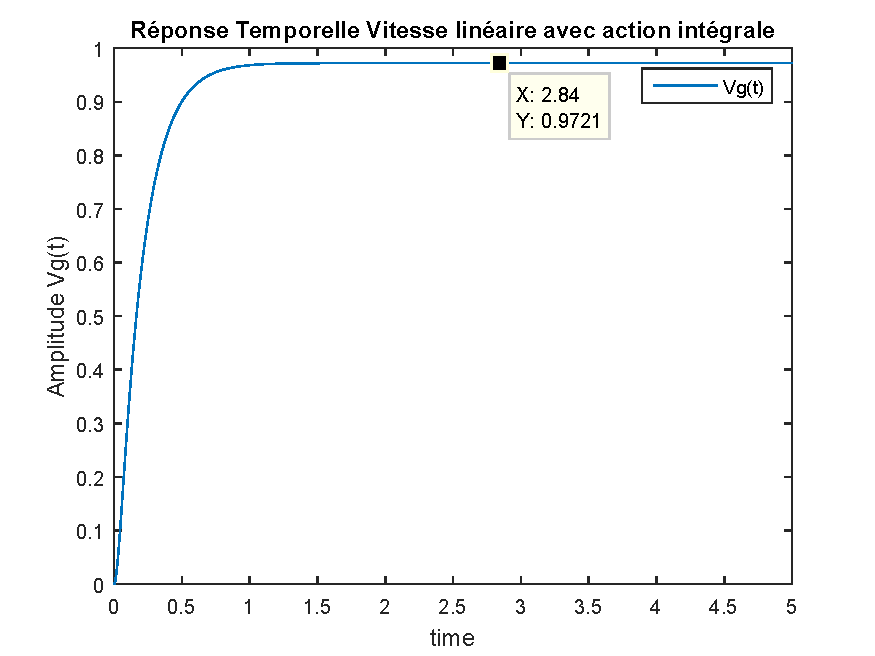
\includegraphics[width = \textwidth]{./IV/images/rep_RI_lineaire5s.pdf}
\caption{Réponse temporelle du système linéaire asservis avec un retour d'état avec action intégrale\label{fig:rep_RI_lineaire}}
\end{minipage}
\begin{minipage}{.5\textwidth}
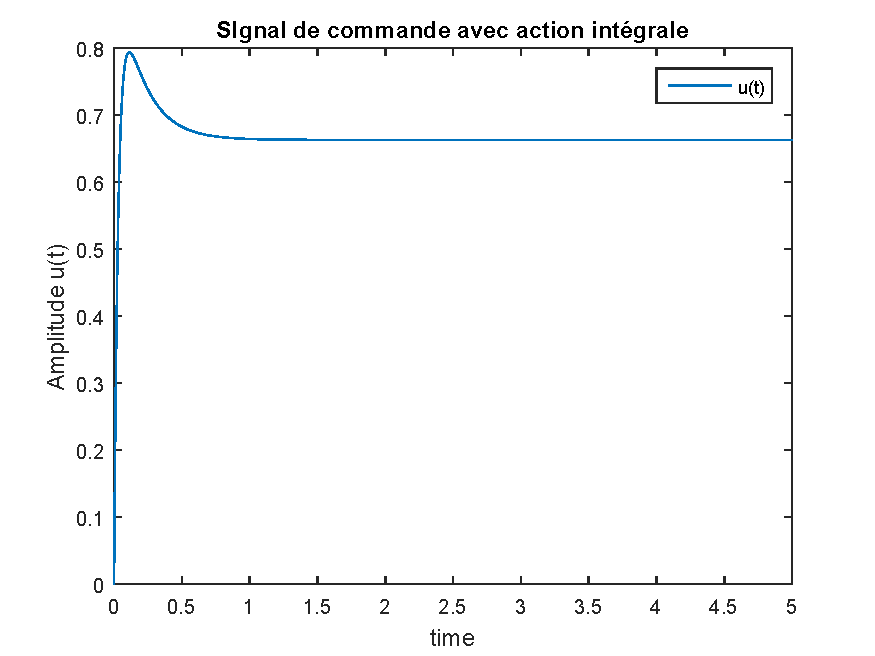
\includegraphics[width = \textwidth]{./IV/images/com_RI_lineaire5s.pdf}
\caption{Commande du système linéaire asservis avec un retour d'état avec action intégrale\label{fig:com_RI_lineaire}}
\end{minipage}
\end{figure}
		Dans ces réponses simulés, nous observons toujours une erreur de position en régime statique.
\begin{align*}\label{eqn:erreurML_RI}
\epsilon_y = y_{mes_{statique}} - y_{ref} = 0.03 \text{ donc : }\epsilon = 3\%
\end{align*}
Comme nous le disions précédemment, le signal utilisé pour faire converger de l'erreur du régime statique est un signal reconstitué grâce à l'observateur. Cependant, il prend aussi les inconvénients de celui ci. Nous avions remarqué que l'observateur disposait d'une dynamique de reconstruction erroné(\ref{sub:etudeTransfertErreurCommande}), nous la retrouvons ici dans cette simulation.
		La commande appliquée est tout à fait convenable, elle ne dépasse pas la référence ce qui signifie qu'il est possible d'augmenter cette référence. Le temps de réponse n'a pas pu être mesuré correctement, cependant les observations de la figure \ref{fig:rep_RI_lineaire} nous montrent que le régime statique est atteint quand la simulation dépasse les 1 seconde.
		\subsubsection{Prototype 2}
		Nous avons choisi de mettre ce nouveau l'asservissement dans un nouveau prototype. Il est donc composé d'un retour d'état avec une action intégrale. Pour le valider, nous allons maintenant le simuler sur le modèle non linéaire qui a été introduit pour les deux premiers prototypes. Nous pouvons observer les résultats sur les deux figures \ref{fig:rep_RI_Nonlineaire} pour le signal de performances $Vg(t)$ et \ref{fig:com_RI_Nonlineaire} pour la commande $u(t)$ qui est envoyé dans le procédé non linéaire.
		\begin{figure}[!ht]
		\begin{minipage}{.5\textwidth}
		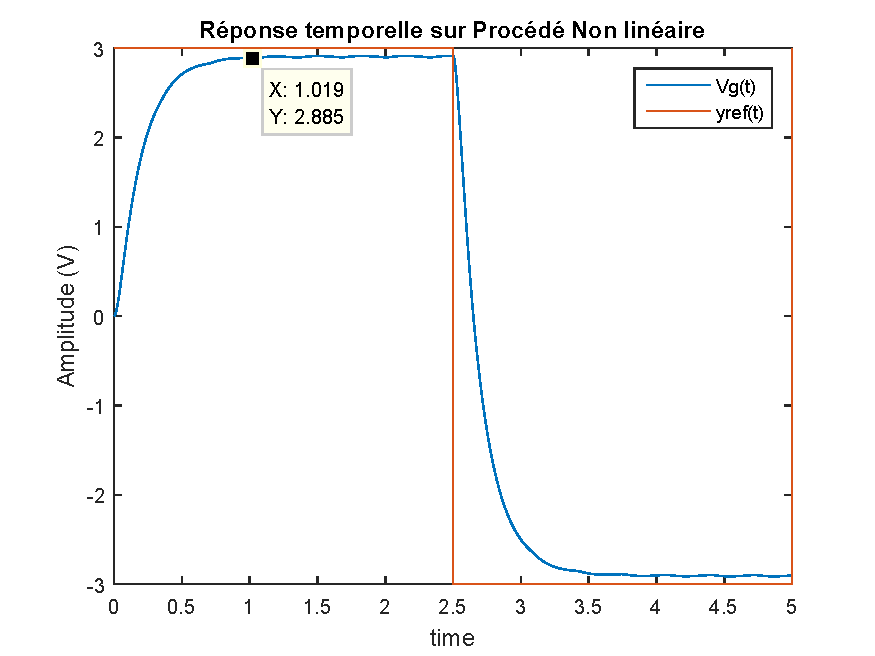
\includegraphics[width = \textwidth]{./IV/images/rep_RI_NonLineaire.pdf}
		\caption{Réponse temporelle du système Non linéaire asservis avec un retour d'état avec action intégrale\label{fig:rep_RI_Nonlineaire}}
\end{minipage}
\begin{minipage}{.5\textwidth}
\includegraphics[width = \textwidth]{./IV/images/com_RI_Nonlineaire.pdf}
\caption{Commande du système Non linéaire asservis avec un retour d'état avec action intégrale\label{fig:com_RI_Nonlineaire}}
\end{minipage}
		\end{figure}
		Sur ces courbes, nous pouvons noter que l'erreur du régime statique est, cette fois ci, $\epsilon_y = 3 - 2.885 = 0.115$, soit, $\epsilon = 3.8\%$. Cette valeur est inférieure à tous les prototypes testés jusqu'à présent, il s'agit donc du meilleur prototype en régime permanent. Le temps de monté est lui aussi respecté et nous n'avons pas d'oscillations. Nous pouvons juger notre commande comme valide.
		\subsection{Conclusion et Validation}
	Les 3 prototypes qui ont sont ressortis du \emph{Model in the loop} n'ont pas tous la même valeurs. Nous avons donc un prototype 0 qui est possède un observateur avec de mauvaises valeurs propres. Nous avons aussi un autre prototype qui lui dispose d'un bonne dynamique en régime transitoire mais n'a pas de bon régime permanent. Enfin, le prototype 2, dispose aussi d'un très bon régime transitoire mais il n'attend pas l'idéal d'une erreur nulle en régime permanent. 
	
	
	
	
%%% Partie sur le moteur Réel	
\section{Simulation sur moteur Réel}
		Nous souhaitons maintenant améliorer nos prototypes avec le banc moteur directement. En utilisant la fonction de prototypage rapide de $MATLAB$, nous sommes capables de générer une émulation du micro contrôleur. Celui ci va s'occuper de récupérer les sorties mesurées du banc moteur, calculer la commande correspondantes et la générer sur l'entrée de commande du moteur. Cette partie va utiliser le protocole $SIL$ décrit en début de chapitre.
		\subsection{Adaptation du modèle}
Pour cette étude, nous avons réutilisé le bloc de simulation utilisé pour le $MIL$. Nous le connectons au bloc conçu pour envoyer et recevoir des signaux analogiques de la carte E/S. Ensuite, un $build$ de la simulation complète est nécessaire pour ensuite lancer une émulation de la commande en temps réel. Vous trouverez le schéma $SIMULINK$ que nous avons utilisé en annexe, figure (\ref{fig:schemaSIMU_MoteurReel}).
		\subsection{Test et étude de performances}
		Nous avons à notre disposition plusieurs prototypes déjà étudié en $MIL$. Cependant, nous n'utiliserons que les prototypes 1 et 2, qui disposent des meilleurs performances. Pour cette partie, nous souhaitons surtout analyser si les contraintes de temps réel sont respectés. Nous sommes dans une émulation, c'est à dire que chaque temps, entre la réception et l'émission est compté.
		
		%Par des soucis de mise en place de test et d'accès au matériel, nous avons été capables d'itérer une seule fois la boucle du $SIL$, sur le prototype 1. Nous aurions aimé pouvoir validé le prototype 2
		\subsubsection{$SIL$ du Prototype 1}		
		% Prototype 1
		Les résultats obtenus sur l'émulation de la commande du prototype 1 vont vous être présentés dans cette partie. Nous avons, pour la 
		\begin{figure}[!ht]
		\centering
		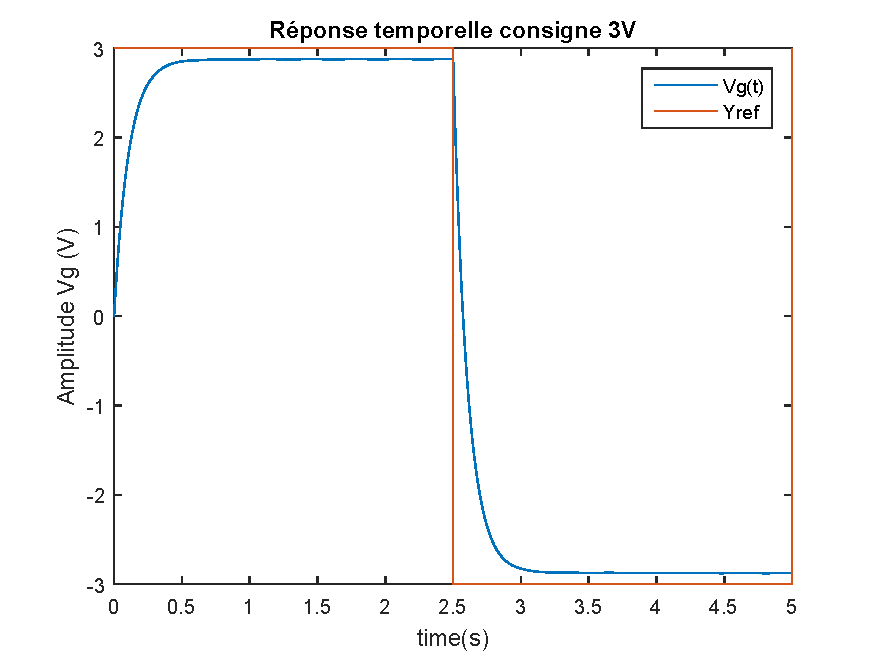
\includegraphics[width = .7\textwidth]{./IV/images/repNL_proto1.pdf}
		\caption{Réponse teporelle $V_g(t)$, commande émulé et procédé réel\label{fig:rep_MoteurReel_proto1}}
\end{figure}				
		\subsection{Conclusion et Validation}
		
%\chapter{Planification de la suite de l'asservissement}
%\label{chap:suite}
%Dans ce chapitre, nous allons décrire les étapes suivantes à cette étude théorique. Dans un premier temps sera présenté la validation de notre commande par tests puis il sera abordé les étapes nécessaires à l'implémentation sur micro-contrôleur et la validation finale.
%\section{Validation de commande}
%Dans un premier temps, nous testerons notre asservissement sur un modèle plus riche (non linéaire, variant, plus de dynamique, ...) en simulation afin de voir si notre commande respecte toujours le cahier des charges. Le modèle sera fournie en seconde séance de TP. Ensuite, nous testerons le moteur dans différentes configurations en fonction des résultats et de notre vitesse d'avancement : 
%\begin{itemize}
%\item Émulation sur le même ordinateur (test du temps concret).
%\item Test de la commande et du procédé sur un même ordinateur en sortant le signal de commande par les cartes d'entrées/sorties du prototypage rapide.
%\item Test de la commande simulée sur un ordinateur et le procédé simulé sur un second ordinateur afin de tester deux vitesses de fonctionnement de simulation (synchronisations) et les cartes entrées/sorties (communications).
%\item Test de la commande simulée et le procédé simulé sur un micro-contrôleur.
%\item Test de la commande simulée sur procédé réel : on éprouve ici la robustesse de la commande face aux imprécisions de modélisation.
%\end{itemize}
%Nous effectuerons aussi une estimation du modèle de comportement du moteur que nous asservirons afin d'avoir un modèle plus proche du comportement réel.
%\section{Implémentation sur micro-contrôleur}
%% CAN CNA
%% Fech et F micro c
%% MODELE Z 
%% PROG
%% ORDO
%% IMPLE
%
%Dans cette partie, nous appréhenderons les problématiques de conversions de signaux numériques/analogiques et analogiques/numériques et essaierons de les corriger afin d'avoir des conversions les plus linéaires possibles. Nous calculerons les fréquences maximales et minimales des entrées et sorties du procédé, cela nous permettra de choisir des fréquences de conversions adaptées et la fréquence de fonctionnement du micro-contrôleur. Nous transformerons aussi notre modèle de commande en un modèle à temps discret afin de pouvoir l'implémenter. Une fois le modèle temps discret obtenu, nous programmerons les différentes fonctions nécessaires à l'asservissement (lecture des entrées, calcul des sorties, écriture des sorties). Nous aborderons aussi les problématiques d'ordonnancement afin que notre programme puisse s'exécuter dans le temps impartie afin de respecter les contraintes temps réels. Enfin, nous implémenterons notre programme sur le micro-contrôleur C167.
%\section{Validation finale}
%Une fois la commande implémentée, nous effectuerons les tests suivants : 
%\begin{itemize}
%\item Test de la commande implémentée sur le procédé simulé sur ordinateur.
%\item Test de la commande implémentée sur le procédé simulé sur micro-contrôleur.
%\item Test de la commande implémentée sur la maquette du procédé réel.
%\end{itemize}
%
%Nous vérifierons le respect des spécifications du cahier des charges dans l'ensemble de ces tests afin de voir si notre asservissement est correct.